\documentclass[12pt, a4paper]{report}

% ─── Packages ────────────────────────────────────────────────────────────────
\usepackage[utf8]{inputenc}
\usepackage[T1]{fontenc}
\usepackage{lmodern}
\usepackage[english]{babel}
\usepackage{geometry}
\usepackage{graphicx}
\usepackage{adjustbox}
\usepackage{amsmath, amssymb}
\usepackage{booktabs}
\usepackage{array}
\usepackage{hyperref}
\usepackage{setspace}
\usepackage{titlesec}
\usepackage{fancyhdr}
\usepackage{tocloft}
\usepackage{xcolor}
\usepackage{listings}
\usepackage{caption}
\usepackage{subcaption}
\usepackage{enumitem}
\usepackage{parskip}
\usepackage{float}
\usepackage{cite}
\usepackage{tikz}
\usepackage{tikz-cd}
\usetikzlibrary{shapes.geometric, arrows.meta, positioning, calc, fit, backgrounds}

% ─── Page geometry ───────────────────────────────────────────────────────────
\geometry{
  top=2.5cm, bottom=2.5cm,
  left=3cm,  right=2.5cm
}

% ─── Spacing ─────────────────────────────────────────────────────────────────
\onehalfspacing

% ─── Colors ──────────────────────────────────────────────────────────────────
\definecolor{vnuBlue}{RGB}{0, 70, 127}
\definecolor{accentRed}{RGB}{180, 30, 30}
\definecolor{codeGray}{RGB}{245, 245, 245}
\definecolor{commentGreen}{RGB}{60, 128, 49}
\definecolor{pipeBlue}{RGB}{220, 235, 247}
\definecolor{pipeArrow}{RGB}{0, 100, 180}

% ─── Hyperref setup ──────────────────────────────────────────────────────────
\hypersetup{
  colorlinks = true,
  linkcolor  = vnuBlue,
  citecolor  = accentRed,
  urlcolor   = vnuBlue,
  pdftitle   = {Video Summarization by Supervised Learning -- Proposal},
  pdfauthor  = {Tran Hai Duc}
}

% ─── Header / Footer ─────────────────────────────────────────────────────────
\pagestyle{fancy}
\fancyhf{}
\fancyhead[L]{\footnotesize\textit{Video Summarization by Supervised Learning}}
\fancyhead[R]{\footnotesize\textit{Duc (23127173) \& Chien (23127331)}}
\fancyfoot[C]{\thepage}
\renewcommand{\headrulewidth}{0.4pt}

% ─── Section title formatting ─────────────────────────────────────────────────
\titleformat{\chapter}[display]
  {\normalfont\Large\bfseries\color{vnuBlue}}
  {\chaptertitlename\ \thechapter}{10pt}{\huge}
\titlespacing*{\chapter}{0pt}{30pt}{20pt}

\titleformat{\section}
  {\normalfont\large\bfseries\color{vnuBlue}}
  {\thesection}{1em}{}

\titleformat{\subsection}
  {\normalfont\normalsize\bfseries}
  {\thesubsection}{1em}{}

% ─── Code listing style ───────────────────────────────────────────────────────
\lstset{
  backgroundcolor=\color{codeGray},
  basicstyle=\small\ttfamily,
  breaklines=true,
  commentstyle=\color{commentGreen},
  keywordstyle=\bfseries\color{vnuBlue},
  numbers=left,
  numberstyle=\tiny\color{gray},
  frame=single,
  captionpos=b
}

% ─── TikZ styles for pipeline diagrams ───────────────────────────────────────
\tikzset{
  pipenode/.style={
    rectangle, rounded corners=4pt,
    draw=vnuBlue, fill=pipeBlue,
    text width=3.2cm, minimum height=1.0cm,
    align=center, font=\small\bfseries
  },
  pipenarrow/.style={
    ->, >=latex, thick, color=pipeArrow
  },
  ionode/.style={
    rectangle, rounded corners=4pt,
    draw=accentRed, fill=accentRed!10,
    text width=2.8cm, minimum height=0.8cm,
    align=center, font=\small
  },
  dimnode/.style={
    rectangle,
    draw=gray!60, fill=gray!10,
    text width=2.4cm, minimum height=0.7cm,
    align=center, font=\footnotesize\ttfamily
  },
  block/.style={
    rectangle,
    rounded corners=5pt,
    draw=vnuBlue!85!black,
    fill=pipeBlue!70,
    minimum width=3.0cm,
    minimum height=1.1cm,
    align=center,
    font=\small\bfseries
  },
  dim/.style={
    rectangle,
    draw=gray!60,
    fill=gray!12,
    minimum width=3.0cm,
    minimum height=0.45cm,
    align=center,
    font=\scriptsize\ttfamily
  },
  arrow/.style={
    -{Stealth[length=3mm,width=2mm]},
    very thick,
    color=pipeArrow
  }
}

% ─────────────────────────────────────────────────────────────────────────────
%  DOCUMENT
% ─────────────────────────────────────────────────────────────────────────────
\begin{document}

% ════════════════════════════════════════════════════════════════════════════
%  COVER PAGE
% ════════════════════════════════════════════════════════════════════════════
\begin{titlepage}
\thispagestyle{empty}
\begin{center}

  {\large\textbf{VIETNAM NATIONAL UNIVERSITY -- HO CHI MINH CITY}}\\[4pt]
  {\large\textbf{UNIVERSITY OF SCIENCE}}\\[4pt]
  {\large\textbf{FACULTY OF INFORMATION TECHNOLOGY}}

  \vspace{1.5cm}
  \hrule height 1.2pt
  \vspace{0.4cm}
  \hrule height 0.4pt
  \vspace{1.5cm}

  {\color{vnuBlue}\Huge\bfseries
    Video Summarization\\[8pt]
    by Supervised Learning
  }

  \vspace{0.8cm}
  {\Large\bfseries Research Proposal}

  \vspace{0.5cm}
  \hrule height 0.4pt
  \vspace{0.4cm}
  \hrule height 1.2pt
  \vspace{1.8cm}

  \begin{minipage}{0.48\textwidth}
    \raggedright
    \textbf{Students:}\\[4pt]
    \quad Tran Hai Duc\\
    \quad Student ID: \texttt{23127173}\\[6pt]
    \quad Nguyen Cong Chien\\
    \quad Student ID: \texttt{23127331}
  \end{minipage}
  \hfill
  \begin{minipage}{0.48\textwidth}
    \raggedleft
    \textbf{Supervisor:}\\[4pt]
    Vo Hoai Viet, Ph.D.
  \end{minipage}

  \vfill

  {\large Ho Chi Minh City, \the\year}

\end{center}
\end{titlepage}

% ════════════════════════════════════════════════════════════════════════════
%  ACKNOWLEDGEMENTS
% ════════════════════════════════════════════════════════════════════════════
\chapter*{Acknowledgements}
\addcontentsline{toc}{chapter}{Acknowledgements}
\thispagestyle{fancy}

First and foremost, we would like to express our sincere gratitude to our supervisor,
\textbf{Dr.\ Vo Hoai Viet}, for his invaluable guidance, encouragement, and continuous
support throughout this research project. His insightful feedback, deep expertise in
computer vision and machine learning, and willingness to create a conducive research
environment have been instrumental in shaping both the direction and the quality of
this work.

We also wish to extend our heartfelt thanks to the research community whose open
contributions have made this study possible. The authors of the \textbf{SumMe} and
\textbf{TVSum} benchmark datasets provided critical evaluation resources that enabled
rigorous experimentation. The developers of \textbf{OpenAI Whisper}, \textbf{SentenceBERT},
and the underlying pre-trained deep learning models offered foundational building blocks
without which the proposed pipeline could not be realised.

Special thanks go to all classmates and friends for their moral support and stimulating
discussions during challenging moments of the research process. Finally, we are deeply
indebted to our families for their unwavering love, patience, and encouragement
throughout our studies.

\vspace{1.5cm}
\begin{flushright}
  \textit{Ho Chi Minh City, \the\year}\\[6pt]
  \textit{Tran Hai Duc \& Nguyen Cong Chien}
\end{flushright}

\newpage

% ════════════════════════════════════════════════════════════════════════════
%  TABLE OF CONTENTS
% ════════════════════════════════════════════════════════════════════════════
\tableofcontents
\newpage

% ════════════════════════════════════════════════════════════════════════════
%  CHAPTER 1 -- INTRODUCTION
% ════════════════════════════════════════════════════════════════════════════
\chapter{Introduction}

\section{Overview of Video Summarization}

\textbf{Video summarization} is the task of automatically generating a compact
representation of a video that retains its most important content and storyline
\cite{haq2021,money2015}. Depending on the output format, summaries fall into two
main categories:

\begin{itemize}[leftmargin=1.5cm]
  \item \textbf{Static summary:} a set of representative keyframes extracted from
        the original video.
  \item \textbf{Dynamic summary:} a shortened video clip assembled from selected
        important segments, preserving both visual content and audio.
\end{itemize}

The overarching goal is to \emph{reduce viewing time} without sacrificing the essential
narrative, allowing users to grasp the key content efficiently.

\section{Motivating Examples}

\subsection{Everyday Use Case}
Consider a user who wishes to watch a one-hour lecture on YouTube but has only ten
minutes available. A video summarization system can automatically identify segments
containing core explanations, motivating examples, and concluding remarks, then
assemble a condensed version of approximately 6--10 minutes, enabling the user to
absorb 70--80\,\% of the essential content without watching the full hour.

\subsection{Data Reduction Perspective}
In \textbf{video classification} tasks, models must process thousands of frames per
video, incurring large computational costs. By first summarizing a video to retain
only $\approx 15\,\%$ of its frames, the downstream classifier effectively operates on
a lower-dimensional representation, yielding reduced computation and storage requirements
while focusing on information-rich frames.

\section{Significance of the Work}

\subsection{Practical Significance}
The practical impact of video summarization includes \cite{kadam2022}:
\begin{itemize}[leftmargin=1.5cm]
  \item \textbf{Time savings for users:} viewers can quickly understand the content
        of long videos without watching them in full.
  \item \textbf{Support for recommendation and retrieval:} meaningful keyframes improve
        thumbnail generation and enable preview functionality.
  \item \textbf{Applications in education and news:} automatic highlight extraction
        for lectures, MOOCs, and broadcast news programmes.
\end{itemize}

\subsection{Scientific Significance}
\begin{itemize}[leftmargin=1.5cm]
  \item \textbf{Structured dimensionality reduction:} video summarization selects
        frames or segments with high \emph{information content}, rather than applying
        uniform down-sampling.
  \item \textbf{Pre-processing for downstream models:} summarizing large video corpora
        before training classification, retrieval, or captioning models reduces
        training costs and focuses learning on informative data.
\end{itemize}

\section{Research Context}

Current approaches to video summarization span a wide spectrum \cite{apostolidis2021}:
\begin{itemize}[leftmargin=1.5cm]
  \item \textbf{Traditional methods:} heuristic rules, clustering, shot detection.
  \item \textbf{Deep learning:} sequence labeling with LSTM/BiLSTM \cite{zhang2016},
        attention and Transformer models, reinforcement learning, self-supervised learning.
  \item \textbf{Multimodal methods:} combining visual, audio, transcript, and metadata
        features \cite{psallidas2021,hu2023}.
\end{itemize}

Recent surveys \cite{apostolidis2021} identify several open opportunities:
\begin{itemize}[leftmargin=1.5cm]
  \item Better exploitation of textual and audio signals (speech, subtitles, OCR).
  \item More effective modeling of long sequences using hierarchical Transformers.
  \item Unsupervised and semi-supervised learning to reduce annotation costs.
\end{itemize}

\section{Research Focus}

This project targets \textbf{multimodal video summarization (visual + audio)} in a
supervised setting on the SumMe \cite{gygli2014} and TVSum \cite{song2015} benchmarks.
The proposed architecture combines a \textbf{BiLSTM with Temporal Attention}
\cite{zhang2016} with an audio branch built on Whisper \cite{radford2023} and
SentenceBERT \cite{reimers2019}. The primary deliverable is a \textbf{dynamic summary}
-- a condensed video clip with intact audio.

% ════════════════════════════════════════════════════════════════════════════
%  CHAPTER 2 -- PROBLEM FORMULATION
% ════════════════════════════════════════════════════════════════════════════
\chapter{Problem Formulation}

\section{Input}

\begin{itemize}[leftmargin=1.5cm]
  \item A raw video $V$ in any standard container format (\texttt{.mp4}, \texttt{.avi},
        etc.) of arbitrary duration.
  \item During training: frame-level importance scores $y_t \in [0,1]$ for each frame
        $t$, derived from human annotations provided in the SumMe and TVSum datasets.
\end{itemize}

\section{Output}

\begin{itemize}[leftmargin=1.5cm]
  \item \textbf{Static summary:} a set of representative keyframes that collectively
        depict the video's main content.
  \item \textbf{Dynamic summary:} a condensed video $V_{\text{sum}}$ of approximately
        $35\,\%$ of the original duration, assembled from the most important segments
        and retaining the corresponding audio track.
\end{itemize}

\section{Implementation Focus}

This project concentrates on \textbf{dynamic summaries} for three reasons:
\begin{enumerate}[leftmargin=1.5cm]
  \item They more closely match real-world user needs -- watching a short video with
        sound rather than browsing static images.
  \item They allow qualitative evaluation through direct viewing experience.
  \item They fully exploit the \texttt{ffmpeg}-based audio processing pipeline
        developed in this project.
\end{enumerate}

Static keyframe export is also supported as a by-product of the keyshot selection step.

% ════════════════════════════════════════════════════════════════════════════
%  CHAPTER 3 -- METHODOLOGY
% ════════════════════════════════════════════════════════════════════════════
\chapter{Methodology}

\section{Supervised Learning Framework}

The model learns to approximate human importance judgements:
\begin{itemize}[leftmargin=1.5cm]
  \item \textbf{Input:} a sequence of multimodal feature vectors
        $\{x_t\}_{t=1}^{T}$, $x_t \in \mathbb{R}^{2432}$.
  \item \textbf{Output:} raw logits $z_t \in \mathbb{R}$ for each frame $t$;
        probabilities $\hat{y}_t = \sigma(z_t) \in [0,1]$ are recovered via sigmoid
        (applied implicitly inside the loss during training).
  \item \textbf{Ground truth:} $y_t \in [0,1]$, the mean score assigned by 15--20
        human annotators, binarised at threshold $0.5$ for loss computation.
  \item \textbf{Loss:} Binary Cross-Entropy with Logits (\texttt{BCEWithLogitsLoss}),
        which combines a sigmoid activation with binary cross-entropy in a numerically
        stable single operation:
        \begin{equation}
          \mathcal{L} = -\frac{1}{T}\sum_{t=1}^{T}
            \bigl[y_t \log\sigma(z_t) + (1-y_t)\log(1-\sigma(z_t))\bigr]
        \end{equation}
\end{itemize}

\section{Datasets}

\subsection{SumMe \cite{gygli2014}}
SumMe is a collection of short, thematically diverse user-generated videos.
Annotators manually mark important segments; these are converted to frame-level
importance scores used as ground truth.

\subsection{TVSum \cite{song2015}}
TVSum is oriented toward ``TV program'' content (news, documentaries, vlogs). Each
video is annotated by approximately 20 raters; the mean score constitutes the ground
truth.

\section{Evaluation Metrics}

\begin{itemize}[leftmargin=1.5cm]
  \item \textbf{F-score} (F-measure): measures temporal overlap between the generated
        summary and the annotator-derived reference summary.
  \item \textbf{Precision / Recall:}
        \begin{itemize}
          \item \emph{Precision} -- proportion of summary content that is genuinely important.
          \item \emph{Recall} -- proportion of important video content retained in the summary.
        \end{itemize}
  \item \textbf{Temporal Overlap:} degree of time-segment overlap between predicted
        summary segments and ground-truth segments.
\end{itemize}

% ════════════════════════════════════════════════════════════════════════════
%  CHAPTER 4 -- PROPOSED ARCHITECTURE
% ════════════════════════════════════════════════════════════════════════════
\chapter{Proposed Architecture: Multimodal BiLSTM with Temporal Attention}

\section{Architecture Overview}

Figure~\ref{fig:arch_overview} shows the end-to-end architecture. Two parallel
branches extract visual and audio features, which are fused at the frame level before
being fed into the BiLSTM--Temporal Attention stack that produces per-frame
importance scores.

\begin{figure}[t]
\centering
\begin{adjustbox}{max width=\textwidth}
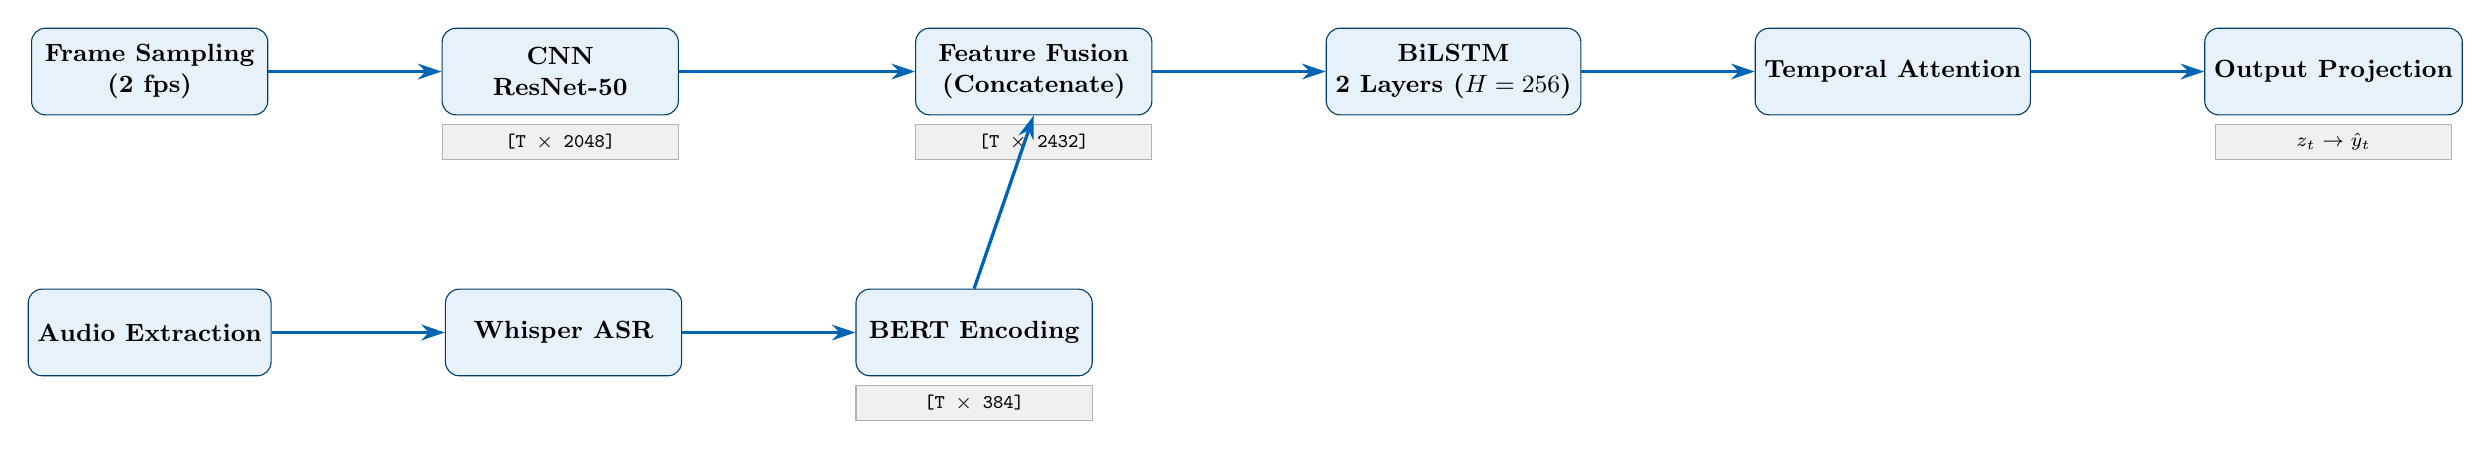
\begin{tikzpicture}[
  node distance = 2.2cm and 2.2cm,
  >=Stealth
]

% --- Video branch ---
\node[block] (frames) {Frame Sampling\\(2 fps)};
\node[block, right=of frames] (cnn) {CNN\\ResNet-50};
\node[dim, below=3pt of cnn] {[T $\times$ 2048]};

% --- Audio branch ---
\node[block, below=2.2cm of frames] (audio) {Audio Extraction};
\node[block, right=of audio] (whisper) {Whisper ASR};
\node[block, right=of whisper] (bert) {BERT Encoding};
\node[dim, below=3pt of bert] {[T $\times$ 384]};

% --- Fusion ---
\node[block, right=3cm of cnn] (fusion) {Feature Fusion\\(Concatenate)};
\node[dim, below=3pt of fusion] {[T $\times$ 2432]};

% --- Sequence ---
\node[block, right=of fusion] (bilstm) {BiLSTM\\2 Layers ($H=256$)};
\node[block, right=of bilstm] (attn) {Temporal Attention};
\node[block, right=of attn] (proj) {Output Projection};
\node[dim, below=3pt of proj] {$z_t \rightarrow \hat{y}_t$};

% --- Video arrows ---
\draw[arrow] (frames) -- (cnn);
\draw[arrow] (cnn) -- (fusion);

% --- Audio arrows ---
\draw[arrow] (audio) -- (whisper);
\draw[arrow] (whisper) -- (bert);

% vertical merge (audio branch into fusion)
\draw[arrow] (bert.north) -- (fusion.south);

% --- sequence arrows ---
\draw[arrow] (fusion) -- (bilstm);
\draw[arrow] (bilstm) -- (attn);
\draw[arrow] (attn) -- (proj);

\end{tikzpicture}
\end{adjustbox}
\caption{Multimodal video summarization architecture combining visual and audio pipelines.}
\label{fig:arch_overview}
\end{figure}

\section{BiLSTM Overview}

A \textbf{Bidirectional Long Short-Term Memory (BiLSTM)} network \cite{zhang2016}
processes the input sequence in both the forward (past) and backward (future) temporal
directions. For each frame $t$, the hidden state encodes context from all preceding
frames (forward pass) and all subsequent frames (backward pass).

Formally, given input sequence $(x_1, \dots, x_T)$ with $x_t \in \mathbb{R}^{2432}$:
\begin{equation}
  (h_1, \dots, h_T) = \mathrm{BiLSTM}(x_1, \dots, x_T), \quad h_t \in \mathbb{R}^{2H}
\end{equation}
where $H = 256$ is the hidden size per direction, giving $h_t \in \mathbb{R}^{512}$.

\section{Temporal Attention}

Temporal attention is applied on top of the BiLSTM outputs to focus the model on
the most informative time steps:
\begin{align}
  e_t      &= \tanh\!\bigl(W_h\, h_t + b_h\bigr) \\
  \alpha_t &= \operatorname{softmax}\!\bigl(w^{\top} e_t\bigr)
\end{align}
The weights $\alpha_t$ modulate each frame's contribution when predicting importance
scores, effectively down-weighting noisy or redundant segments.

\section{Frame Importance Prediction}

The output layer is a linear projection (no sigmoid activation) producing raw logits:
\begin{equation}
  z_t = W_o\, h_t + b_o \in \mathbb{R}
\end{equation}
During training, the sigmoid is applied implicitly inside \texttt{BCEWithLogitsLoss}.
At inference, probabilities are recovered as $\hat{y}_t = \sigma(z_t) \in [0,1]$.

\section{Motivation for BiLSTM}

\begin{itemize}[leftmargin=1.5cm]
  \item \textbf{Long-range context:} frame importance depends on temporal context,
        not on local content alone.
  \item \textbf{Bidirectionality:} combining past and future context yields richer
        representations than a unidirectional LSTM.
  \item \textbf{Synergy with attention:} attention weights highlight temporally
        important regions while suppressing irrelevant ones.
\end{itemize}

% ════════════════════════════════════════════════════════════════════════════
%  CHAPTER 5 -- AUDIO PROCESSING PIPELINE
% ════════════════════════════════════════════════════════════════════════════
\chapter{Audio Processing Pipeline}

\section{Overview}

To go beyond visual features, this project incorporates \textbf{speech-derived
semantic embeddings} as an additional modality. The pipeline transforms the raw
audio track into a per-frame feature vector aligned with the visual timeline.
Figure~\ref{fig:audio_pipeline} illustrates the five-step process.

\begin{figure}[H]
\centering
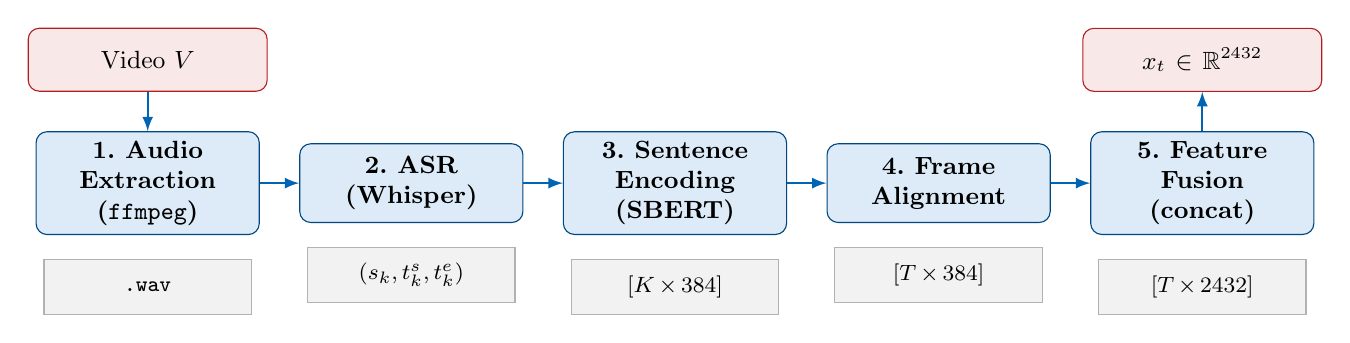
\begin{tikzpicture}[node distance=0.5cm]
  \node[pipenode, text width=2.6cm] (s1) {1.\ Audio\\Extraction\\(\texttt{ffmpeg})};
  \node[pipenode, text width=2.6cm, right=of s1] (s2) {2.\ ASR\\(Whisper)};
  \node[pipenode, text width=2.6cm, right=of s2] (s3) {3.\ Sentence\\Encoding\\(SBERT)};
  \node[pipenode, text width=2.6cm, right=of s3] (s4) {4.\ Frame\\Alignment};
  \node[pipenode, text width=2.6cm, right=of s4] (s5) {5.\ Feature\\Fusion\\(concat)};

  \node[ionode,  above=0.5cm of s1] (inp)  {Video $V$};
  \node[ionode,  above=0.5cm of s5] (out)  {$x_t \!\in\! \mathbb{R}^{2432}$};

  \draw[pipenarrow] (inp) -- (s1);
  \draw[pipenarrow] (s1)  -- (s2);
  \draw[pipenarrow] (s2)  -- (s3);
  \draw[pipenarrow] (s3)  -- (s4);
  \draw[pipenarrow] (s4)  -- (s5);
  \draw[pipenarrow] (s5)  -- (out);

  \node[dimnode, below=0.3cm of s1] {\texttt{.wav}};
  \node[dimnode, below=0.3cm of s2] {$(s_k, t^s_k, t^e_k)$};
  \node[dimnode, below=0.3cm of s3] {$[K\!\times\!384]$};
  \node[dimnode, below=0.3cm of s4] {$[T\!\times\!384]$};
  \node[dimnode, below=0.3cm of s5] {$[T\!\times\!2432]$};
\end{tikzpicture}
\caption{Audio processing pipeline from raw video to frame-level multimodal features.}
\label{fig:audio_pipeline}
\end{figure}

\section{Step-by-Step Description}

\subsection{Step 1 -- Audio Extraction}
The audio track is extracted from the source video using \texttt{ffmpeg}, producing
a \texttt{.wav} file.

\subsection{Step 2 -- Automatic Speech Recognition with Whisper}
OpenAI Whisper \cite{radford2023} transcribes the audio into text segments, each
accompanied by start and end timestamps:
\[
  \text{audio} \;\xrightarrow{\;\text{Whisper}\;}\;
  \bigl\{(\text{sentence}_k,\; t^{\text{start}}_k,\; t^{\text{end}}_k)\bigr\}_{k=1}^{K}
\]

\subsection{Step 3 -- Sentence Encoding with SentenceBERT}
Each transcript sentence is encoded into a dense semantic vector using
SentenceBERT \cite{reimers2019}:
\begin{equation}
  a^{\text{text}}_k = \mathrm{SentenceBERT}(\text{sentence}_k) \in \mathbb{R}^{384}
\end{equation}

\subsection{Step 4 -- Frame-Level Alignment}
Given the timestamp of each sampled frame $t$, the audio embedding is assigned as:
\begin{equation}
  a_t =
  \begin{cases}
    a^{\text{text}}_k & \text{if frame } t \text{ falls within }
                          [t^{\text{start}}_k,\; t^{\text{end}}_k] \\[4pt]
    \mathbf{0}        & \text{otherwise (silence or no speech)}
  \end{cases}
\end{equation}
This produces an audio feature sequence of shape $[T, 384]$, temporally aligned
with the visual feature sequence $[T, 2048]$.

\subsection{Step 5 -- Multimodal Feature Fusion}
Visual and audio features are concatenated at the frame level:
\begin{equation}
  x_t = \bigl[v_t;\; a_t\bigr] \in \mathbb{R}^{2432}
\end{equation}
The resulting sequence $\{x_t\}_{t=1}^{T}$ is the sole input to the BiLSTM.

\section{Benefits of the Audio Branch}
\begin{itemize}[leftmargin=1.5cm]
  \item Enables the model to detect semantically rich spoken content (definitions,
        conclusions, slide titles).
  \item Complements visual features in low-motion segments where important verbal
        explanation occurs over a static slide.
\end{itemize}

% ════════════════════════════════════════════════════════════════════════════
%  CHAPTER 6 -- SYSTEM PIPELINE
% ════════════════════════════════════════════════════════════════════════════
\chapter{System Pipeline}

\section{Training Pipeline}

Figure~\ref{fig:train_pipeline} shows the four phases of the training workflow,
from raw data to a saved model checkpoint.

\begin{figure}[H]
\centering
\begin{adjustbox}{max width=\textwidth}
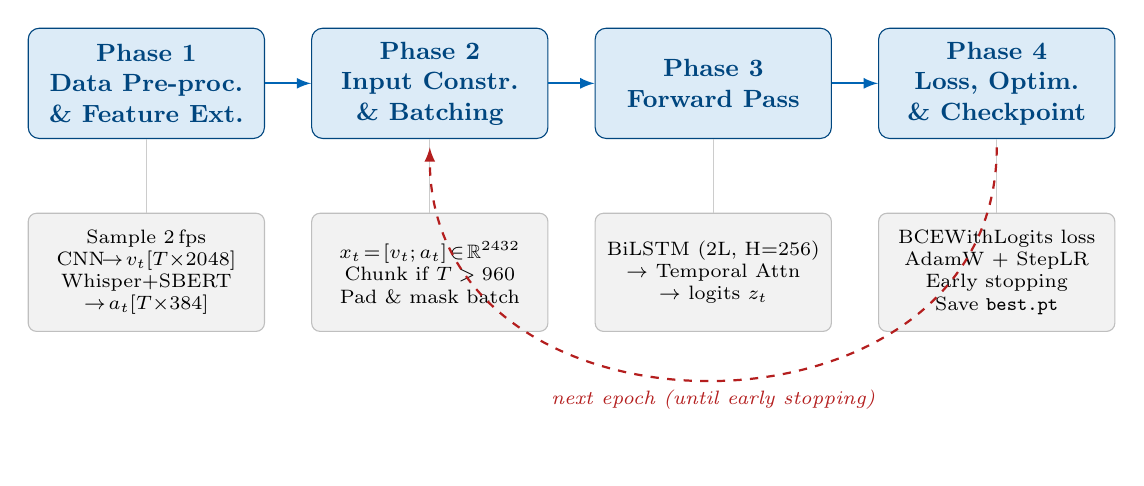
\begin{tikzpicture}[
  phase/.style={rectangle, draw=vnuBlue, fill=pipeBlue, rounded corners=4pt,
                minimum width=3.0cm, minimum height=1.4cm, align=center,
                font=\small\bfseries, text=vnuBlue},
  detail/.style={rectangle, draw=gray!50, fill=gray!10, rounded corners=3pt,
                 minimum width=3.0cm, minimum height=1.5cm, align=center,
                 font=\scriptsize},
  arr/.style={->, >=latex, thick, color=pipeArrow},
  darr/.style={->, >=latex, thick, dashed, color=accentRed}
]
  % x positions for 4 phases (equally spaced, 3.6cm apart)
  \def\xa{0.0}  \def\xb{3.6}  \def\xc{7.2}  \def\xd{10.8}
  \def\ytop{0}  \def\ybot{-2.4}

  % Phase boxes (top row)
  \node[phase] (p1) at (\xa, \ytop)
    {\textbf{Phase 1}\\Data Pre-proc.\\\& Feature Ext.};
  \node[phase] (p2) at (\xb, \ytop)
    {\textbf{Phase 2}\\Input Constr.\\\& Batching};
  \node[phase] (p3) at (\xc, \ytop)
    {\textbf{Phase 3}\\Forward Pass};
  \node[phase] (p4) at (\xd, \ytop)
    {\textbf{Phase 4}\\Loss, Optim.\\\& Checkpoint};

  % Detail boxes (bottom row)
  \node[detail] (d1) at (\xa, \ybot)
    {Sample 2\,fps\\CNN$\!\to\!v_t[T{\times}2048]$\\Whisper+SBERT\\$\to\!a_t[T{\times}384]$};
  \node[detail] (d2) at (\xb, \ybot)
    {$x_t\!=\![v_t;a_t]\!\in\!\mathbb{R}^{2432}$\\Chunk if $T>960$\\Pad \& mask batch};
  \node[detail] (d3) at (\xc, \ybot)
    {BiLSTM (2L, H=256)\\$\to$ Temporal Attn\\$\to$ logits $z_t$};
  \node[detail] (d4) at (\xd, \ybot)
    {BCEWithLogits loss\\AdamW + StepLR\\Early stopping\\Save \texttt{best.pt}};

  % Forward arrows between phases
  \draw[arr] (p1) -- (p2);
  \draw[arr] (p2) -- (p3);
  \draw[arr] (p3) -- (p4);

  % Connectors phase → detail (vertical dotted lines)
  \draw[gray!40, thin] (p1.south) -- (d1.north);
  \draw[gray!40, thin] (p2.south) -- (d2.north);
  \draw[gray!40, thin] (p3.south) -- (d3.north);
  \draw[gray!40, thin] (p4.south) -- (d4.north);

  % Feedback loop arrow (validation / next epoch)
  \draw[darr]
    ([yshift=-3pt]p4.south)
      to[out=-90, in=-90, looseness=1.4]
    node[midway, below, font=\scriptsize\itshape, color=accentRed]
      {next epoch (until early stopping)}
    ([yshift=-3pt]p2.south);

\end{tikzpicture}
\end{adjustbox}
\caption{Training pipeline: from raw video to optimised model checkpoint.}
\label{fig:train_pipeline}
\end{figure}

\subsection{Phase 1 -- Data Pre-processing and Feature Extraction}

Frames are sampled at 2\,fps using a \texttt{FrameSampler}. A pre-trained
\textbf{ResNet-50} CNN extracts a feature vector for each frame:
\[
  v_t = \mathrm{CNN}(f_t) \in \mathbb{R}^{2048}
\]
Features are stored as \texttt{\{video\_id\}.npy} with shape $[T, 2048]$.
Audio features of shape $[T, 384]$ are stored as \texttt{\{video\_id\}\_audio.npy},
following the pipeline of Chapter~5.

\subsection{Phase 2 -- Input Construction and Batching}

For each frame $t$: $x_t = [v_t;\, a_t] \in \mathbb{R}^{2432}$.
Videos longer than \texttt{max\_seq\_len} (960 frames) are chunked.
A \texttt{DataLoader} shuffles videos/segments, pads sequences within each
mini-batch, and applies loss masking on padding positions.

\subsection{Phase 3 -- Forward Pass}

The sequence $\{x_t\}$ is processed by:
\begin{enumerate}[leftmargin=1.5cm]
  \item \textbf{BiLSTM encoding} (2 layers, hidden size 256 per direction).
  \item \textbf{Temporal Attention} to compute per-frame weights $\alpha_t$.
  \item \textbf{Output projection} (linear) to obtain logits $z_t \in \mathbb{R}$.
\end{enumerate}

\subsection{Phase 4 -- Loss Computation and Optimisation}

\paragraph{Supervised Loss.}
The model outputs logits $z_t$; the loss is \textbf{Binary Cross-Entropy with Logits}
(\texttt{BCEWithLogitsLoss}), which folds the sigmoid into the loss for numerical stability:
\begin{equation}
  \mathcal{L} = -\frac{1}{T}\sum_{t=1}^{T}
    \bigl[y_t \log\sigma(z_t) + (1-y_t)\log(1-\sigma(z_t))\bigr]
\end{equation}

\paragraph{Optimiser.}
\textbf{AdamW} with learning rate $\eta = 0.001$ and a \textbf{StepLR} scheduler
(\texttt{step\_size=15}, $\gamma=0.5$). Gradients are back-propagated through the
BiLSTM, attention, and output layers. The best checkpoint is saved to
\texttt{checkpoints/best.pt}; training halts if no improvement is observed for
\texttt{early\_stopping\_patience} consecutive epochs.

\section{Inference / Summary Generation Pipeline}

Figure~\ref{fig:infer_pipeline} illustrates how the trained model is used to produce
a dynamic summary from a new video.

\begin{figure}[H]
\centering
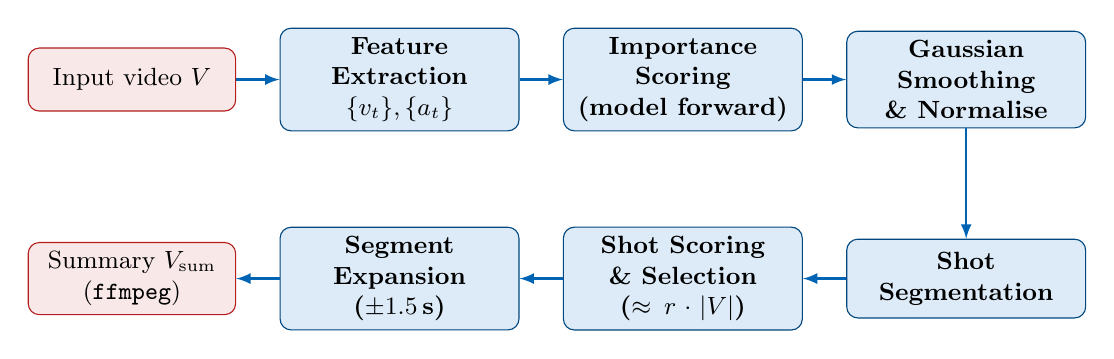
\begin{tikzpicture}[node distance=0.55cm]

  \node[ionode, text width=2.4cm] (vin)   {Input video $V$};

  \node[pipenode, text width=2.8cm, right=of vin] (feat)
    {Feature\\Extraction\\$\{v_t\},\{a_t\}$};

  \node[pipenode, text width=2.8cm, right=of feat] (score)
    {Importance\\Scoring\\(model forward)};

  \node[pipenode, text width=2.8cm, right=of score] (smooth)
    {Gaussian\\Smoothing\\\& Normalise};

  \node[pipenode, text width=2.8cm, below=1.4cm of smooth] (shot)
    {Shot\\Segmentation};

  \node[pipenode, text width=2.8cm, left=of shot] (select)
    {Shot Scoring\\\& Selection\\($\approx r\cdot|V|$)};

  \node[pipenode, text width=2.8cm, left=of select] (expand)
    {Segment\\Expansion\\($\pm1.5$\,s)};

  \node[ionode, text width=2.4cm, left=of expand] (vout)
    {Summary $V_{\text{sum}}$\\(\texttt{ffmpeg})};

  \draw[pipenarrow] (vin)    -- (feat);
  \draw[pipenarrow] (feat)   -- (score);
  \draw[pipenarrow] (score)  -- (smooth);
  \draw[pipenarrow] (smooth) -- (shot);
  \draw[pipenarrow] (shot)   -- (select);
  \draw[pipenarrow] (select) -- (expand);
  \draw[pipenarrow] (expand) -- (vout);

\end{tikzpicture}
\caption{Inference pipeline: from raw video to dynamic summary.}
\label{fig:infer_pipeline}
\end{figure}

\section{Model Hyperparameters}

\begin{table}[H]
\centering
\caption{Model and pipeline hyperparameters}
\label{tab:hyperparams}
\begin{tabular}{ll}
  \toprule
  \textbf{Parameter} & \textbf{Value} \\
  \midrule
  Input dimension      & 2432 (2048 visual + 384 audio) \\
  LSTM hidden size     & 256 (per direction) \\
  LSTM layers          & 2 \\
  Attention            & Temporal Attention \\
  Loss function        & BCEWithLogitsLoss \\
  Optimizer            & AdamW \\
  Learning rate        & 0.001 \\
  LR scheduler         & StepLR (step=15, $\gamma=0.5$) \\
  Frame sampling rate  & 2\,fps \\
  Max sequence length  & 960 frames \\
  Summary ratio $r$    & $\approx 35\,\%$ of original duration \\
  Segment expansion    & $\pm 1.5$\,s \\
  \bottomrule
\end{tabular}
\end{table}

% ════════════════════════════════════════════════════════════════════════════
%  CHAPTER 7 -- EXPECTED RESULTS
% ════════════════════════════════════════════════════════════════════════════
\chapter{Expected Results}

\section{Quantitative Targets}

Table~\ref{tab:expected} presents the expected performance targets on the held-out
test splits of SumMe and TVSum, informed by published results from comparable
supervised methods \cite{apostolidis2021,zhang2016}.

\begin{table}[H]
\centering
\caption{Expected quantitative performance on SumMe and TVSum}
\label{tab:expected}
\begin{tabular}{lccp{5.5cm}}
  \toprule
  \textbf{Metric} & \textbf{SumMe} & \textbf{TVSum} & \textbf{Rationale} \\
  \midrule
  F-score          & $\geq 0.43$ & $\geq 0.55$ & Comparable to LSTM baselines \cite{zhang2016} \\
  Precision        & $\geq 0.42$ & $\geq 0.54$ & Aligned with multimodal method expectations \\
  Recall           & $\geq 0.44$ & $\geq 0.56$ & Sufficient coverage of annotated content \\
  Temporal Overlap & $\geq 0.40$ & $\geq 0.50$ & Meaningful segment alignment with ground truth \\
  \bottomrule
\end{tabular}
\end{table}

\noindent
The audio branch is expected to provide a $+2$--$5\,\%$ F-score gain over a
visual-only BiLSTM baseline, as speech semantics provide complementary signal
for detecting informative segments.

\section{Qualitative Expectations}

The system will be tested on real-world videos of approximately \textbf{10 minutes},
producing dynamic summaries of \textbf{3--4 minutes} ($\approx 35\,\%$ of the
original). Expected characteristics:

\begin{itemize}[leftmargin=1.5cm]
  \item Selected segments concentrate on regions of high activity, meaningful scene
        transitions, and dialogue containing core semantic content.
  \item Shot-based selection combined with Gaussian smoothing and $\pm1.5$\,s context
        expansion is expected to yield visually coherent, low-jitter summaries.
  \item The retained audio track should ensure smooth, uninterrupted sound without
        abrupt cuts.
  \item The overall viewing experience should follow the narrative flow of the
        original video.
\end{itemize}

\section{Ablation Study Plan}

To validate the contribution of each component, we plan the following experiments:

\begin{table}[H]
\centering
\caption{Planned ablation variants}
\label{tab:ablation}
\begin{tabular}{lp{4.5cm}p{4.5cm}}
  \toprule
  \textbf{Variant} & \textbf{Description} & \textbf{Expected Outcome} \\
  \midrule
  Visual-only BiLSTM
    & Remove audio branch; use $v_t \in \mathbb{R}^{2048}$ only
    & Baseline; lower F-score on speech-heavy videos \\[6pt]
  Full model (visual + audio)
    & Use $x_t = [v_t; a_t] \in \mathbb{R}^{2432}$
    & Best performance; audio adds semantic signal \\[6pt]
  No temporal attention
    & BiLSTM without attention weighting
    & Slight drop; attention helps focus on key moments \\[6pt]
  Unidirectional LSTM
    & Forward LSTM only (no backward pass)
    & Reduced context; lower F-score overall \\
  \bottomrule
\end{tabular}
\end{table}

\section{Comparison with Published Baselines}

Upon completion, the proposed model will be benchmarked against:
\begin{itemize}[leftmargin=1.5cm]
  \item \textbf{Zhang et al.\ (2016)} \cite{zhang2016} -- Video summarization with LSTM (visual-only).
  \item \textbf{Apostolidis et al.\ (2021)} \cite{apostolidis2021} -- Survey baselines including
        attention and reinforcement-learning methods.
  \item \textbf{Psallidas et al.\ (2021)} \cite{psallidas2021} -- Multimodal summarization
        (visual + audio).
\end{itemize}

% ════════════════════════════════════════════════════════════════════════════
%  CHAPTER 8 -- PROJECT TIMELINE
% ════════════════════════════════════════════════════════════════════════════
\chapter{Project Timeline}

\section{Overview}

The project is planned over \textbf{5 weeks}, divided into four phases: environment
setup and data preparation, feature extraction and model training, inference pipeline
and evaluation, and final writing and presentation.
Figure~\ref{fig:timeline} presents the Gantt chart; Table~\ref{tab:timeline} lists
the deliverables for each week.

\begin{figure}[H]
\centering
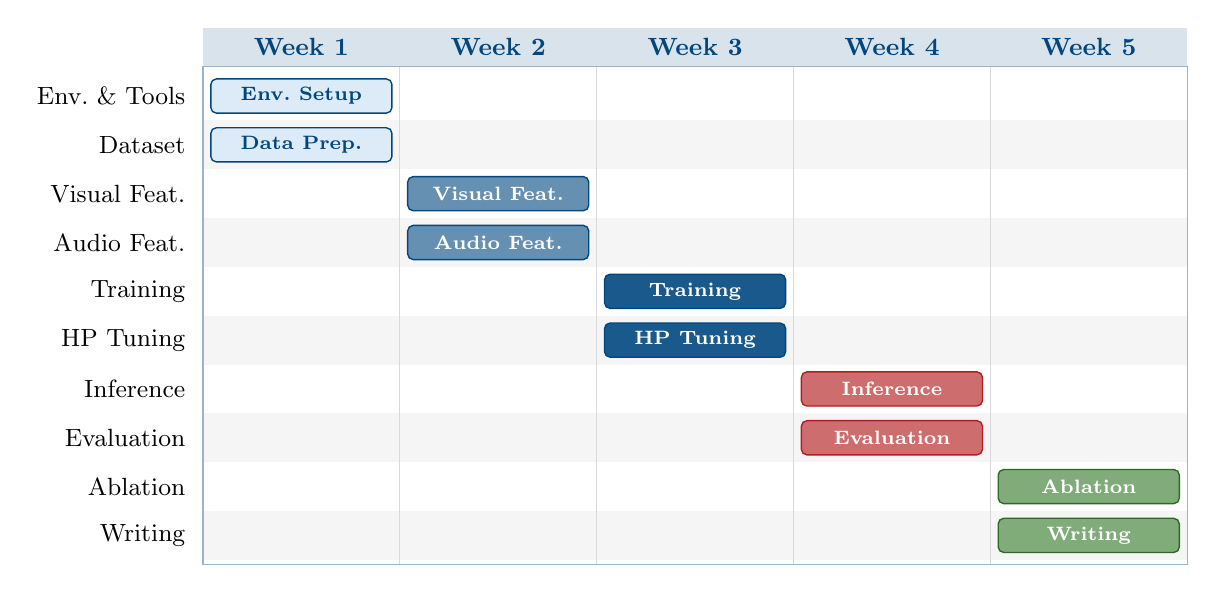
\begin{tikzpicture}[x=1.0cm, y=0.62cm]

  % ── Column header ─────────────────────────────────────────────────────────
  \fill[vnuBlue!15] (2.5,-0.1) rectangle (15.0,-0.9);
  \node[font=\small\bfseries,color=vnuBlue] at (3.75,-0.5) {Week 1};
  \node[font=\small\bfseries,color=vnuBlue] at (6.25,-0.5) {Week 2};
  \node[font=\small\bfseries,color=vnuBlue] at (8.75,-0.5) {Week 3};
  \node[font=\small\bfseries,color=vnuBlue] at (11.25,-0.5) {Week 4};
  \node[font=\small\bfseries,color=vnuBlue] at (13.75,-0.5) {Week 5};

  % ── Alternating row shading ───────────────────────────────────────────────
  \foreach \r in {2,4,6,8,10}{
    \fill[gray!8] (2.5,{-\r}) rectangle (15.0,{-\r-1.0});
  }

  % ── Vertical week separators ──────────────────────────────────────────────
  \foreach \k in {0,1,2,3,4,5}{
    \draw[gray!30,thin] ({2.5+\k*2.5},-0.9) -- ({2.5+\k*2.5},-11.1);
  }

  % ── Row labels ────────────────────────────────────────────────────────────
  \node[anchor=east,font=\small] at (2.4,-1.5) {Env.\ \& Tools};
  \node[anchor=east,font=\small] at (2.4,-2.5) {Dataset};
  \node[anchor=east,font=\small] at (2.4,-3.5) {Visual Feat.};
  \node[anchor=east,font=\small] at (2.4,-4.5) {Audio Feat.};
  \node[anchor=east,font=\small] at (2.4,-5.5) {Training};
  \node[anchor=east,font=\small] at (2.4,-6.5) {HP Tuning};
  \node[anchor=east,font=\small] at (2.4,-7.5) {Inference};
  \node[anchor=east,font=\small] at (2.4,-8.5) {Evaluation};
  \node[anchor=east,font=\small] at (2.4,-9.5) {Ablation};
  \node[anchor=east,font=\small] at (2.4,-10.5) {Writing};

  % ── Week 1 bars ───────────────────────────────────────────────────────────
  \fill[pipeBlue,draw=vnuBlue,line width=0.5pt,rounded corners=2pt]
    (2.6,-1.15) rectangle (4.9,-1.85);
  \node[font=\scriptsize\bfseries,color=vnuBlue] at (3.75,-1.5) {Env.\ Setup};

  \fill[pipeBlue,draw=vnuBlue,line width=0.5pt,rounded corners=2pt]
    (2.6,-2.15) rectangle (4.9,-2.85);
  \node[font=\scriptsize\bfseries,color=vnuBlue] at (3.75,-2.5) {Data Prep.};

  % ── Week 2 bars ───────────────────────────────────────────────────────────
  \fill[vnuBlue!60,draw=vnuBlue,line width=0.5pt,rounded corners=2pt]
    (5.1,-3.15) rectangle (7.4,-3.85);
  \node[font=\scriptsize\bfseries,color=white] at (6.25,-3.5) {Visual Feat.};

  \fill[vnuBlue!60,draw=vnuBlue,line width=0.5pt,rounded corners=2pt]
    (5.1,-4.15) rectangle (7.4,-4.85);
  \node[font=\scriptsize\bfseries,color=white] at (6.25,-4.5) {Audio Feat.};

  % ── Week 3 bars ───────────────────────────────────────────────────────────
  \fill[vnuBlue!90,draw=vnuBlue,line width=0.5pt,rounded corners=2pt]
    (7.6,-5.15) rectangle (9.9,-5.85);
  \node[font=\scriptsize\bfseries,color=white] at (8.75,-5.5) {Training};

  \fill[vnuBlue!90,draw=vnuBlue,line width=0.5pt,rounded corners=2pt]
    (7.6,-6.15) rectangle (9.9,-6.85);
  \node[font=\scriptsize\bfseries,color=white] at (8.75,-6.5) {HP Tuning};

  % ── Week 4 bars ───────────────────────────────────────────────────────────
  \fill[accentRed!65,draw=accentRed,line width=0.5pt,rounded corners=2pt]
    (10.1,-7.15) rectangle (12.4,-7.85);
  \node[font=\scriptsize\bfseries,color=white] at (11.25,-7.5) {Inference};

  \fill[accentRed!65,draw=accentRed,line width=0.5pt,rounded corners=2pt]
    (10.1,-8.15) rectangle (12.4,-8.85);
  \node[font=\scriptsize\bfseries,color=white] at (11.25,-8.5) {Evaluation};

  % ── Week 5 bars ───────────────────────────────────────────────────────────
  \fill[commentGreen!65,draw=commentGreen!80!black,line width=0.5pt,rounded corners=2pt]
    (12.6,-9.15) rectangle (14.9,-9.85);
  \node[font=\scriptsize\bfseries,color=white] at (13.75,-9.5) {Ablation};

  \fill[commentGreen!65,draw=commentGreen!80!black,line width=0.5pt,rounded corners=2pt]
    (12.6,-10.15) rectangle (14.9,-10.85);
  \node[font=\scriptsize\bfseries,color=white] at (13.75,-10.5) {Writing};

  % ── Outer border ─────────────────────────────────────────────────────────
  \draw[vnuBlue!40,thin] (2.5,-0.9) rectangle (15.0,-11.1);

\end{tikzpicture}
\caption{Five-week project Gantt chart.}
\label{fig:timeline}
\end{figure}

\section{Weekly Deliverables}

\begin{table}[H]
\centering
\caption{Weekly tasks and expected deliverables}
\label{tab:timeline}
\begin{tabular}{>{\bfseries}c p{4.2cm} p{5.8cm}}
  \toprule
  \textbf{Week} & \textbf{Tasks} & \textbf{Deliverables} \\
  \midrule
  1
    & Environment setup; library installation; SumMe \& TVSum download and
      format verification
    & Working conda environment; dataset splits in required format;
      \texttt{config.yaml} finalised \\[6pt]
  2
    & ResNet-50 visual feature extraction (2\,fps); Whisper ASR + SentenceBERT
      audio feature extraction; frame-level alignment
    & \texttt{.npy} feature files for all training videos
      ($[T,2048]$ visual, $[T,384]$ audio) \\[6pt]
  3
    & BiLSTM model training with BCEWithLogitsLoss + AdamW + StepLR;
      hyperparameter search (hidden size, learning rate, dropout)
    & Best checkpoint \texttt{best.pt}; training/validation loss curves;
      selected hyperparameter configuration \\[6pt]
  4
    & Inference pipeline (score smoothing, shot segmentation, keyshot
      selection, \texttt{ffmpeg} assembly); quantitative evaluation on
      held-out test split
    & Dynamic summary videos; F-score, precision, recall, and temporal
      overlap results on SumMe \& TVSum \\[6pt]
  5
    & Ablation study (visual-only, no attention, unidirectional LSTM);
      baseline comparison; report writing and slide preparation
    & Ablation result table; comparison with published baselines;
      final report PDF; presentation slides \\
  \bottomrule
\end{tabular}
\end{table}

% ════════════════════════════════════════════════════════════════════════════
%  CHAPTER 9 -- FUTURE WORK
% ════════════════════════════════════════════════════════════════════════════
\chapter{Future Work}

\section{Extending to Multiple Domains}

\begin{enumerate}[leftmargin=1.5cm]
  \item \textbf{Domain-specific video collection:} news broadcasts, educational
        lectures (MOOC/tutorial), and surveillance footage.
  \item \textbf{System evaluation per domain:} apply the current summarization
        pipeline to generate dynamic summaries and record selected keyshot indices
        for downstream use.
\end{enumerate}

\section{Building a Reduced-Dimension Dataset}

The summarized videos will serve as a \emph{structurally reduced} version of the
original corpus. This reduced dataset can train downstream models such as:
\begin{itemize}[leftmargin=1.5cm]
  \item \textbf{Video classification} (topic labeling of news, lecture type, etc.).
  \item \textbf{Video-to-text} (captioning or question answering on condensed video).
\end{itemize}

\section{Downstream Model Integration}

Candidate architectures for training on summarized video:
\begin{itemize}[leftmargin=1.5cm]
  \item \textbf{TimeSformer} -- a Video Vision Transformer with spatiotemporal
        attention, well-suited to shorter, denser sequences produced by summarization.
  \item \textbf{Video Swin Transformer} -- a hierarchical Transformer with 3-D
        shifted windows.
  \item \textbf{I3D / 3D-CNN} -- a simpler baseline for rapid empirical validation.
\end{itemize}

\paragraph{Proposed evaluation protocol.}
\begin{enumerate}[leftmargin=1.5cm]
  \item Use the summarization system to reduce the original corpus by $\approx 85\,\%$.
  \item Assign task labels to the summaries.
  \item Train a downstream model on both original and summarized videos.
  \item Compare classification accuracy, training time, and GPU memory usage.
\end{enumerate}

The central hypothesis is that video summarization \textbf{reduces data dimensionality}
while \textbf{preserving} downstream task performance at lower computational cost.

% ════════════════════════════════════════════════════════════════════════════
%  CHAPTER 9 -- CONCLUSION
% ════════════════════════════════════════════════════════════════════════════
\chapter{Conclusion}

This proposal presents a \textbf{multimodal video summarization system} based on
\textbf{BiLSTM with Temporal Attention} \cite{zhang2016}, combining visual CNN features
with speech-derived semantic embeddings from Whisper \cite{radford2023} and SentenceBERT
\cite{reimers2019}. The system will be trained in a supervised fashion on the SumMe
\cite{gygli2014} and TVSum \cite{song2015} benchmarks, with a target F-score of
$\geq 0.43$ on SumMe and $\geq 0.55$ on TVSum.

Beyond the practical benefit of reducing viewing time, the work demonstrates the role
of video summarization as \textbf{structured dimensionality reduction} -- retaining
information-dense content while discarding redundant frames. This positions the
summarization module as a valuable pre-processing step for downstream video
understanding tasks (classification, retrieval, captioning).

Future directions include a rigorous ablation study and comparison with published
baselines, extension to news and educational domains, and an empirical study of how
summarization-based data reduction affects the performance and efficiency of modern
Transformer-based video classifiers such as TimeSformer.

% ════════════════════════════════════════════════════════════════════════════
%  BIBLIOGRAPHY
% ════════════════════════════════════════════════════════════════════════════
\bibliographystyle{IEEEtran}

\begin{thebibliography}{11}

\bibitem{haq2021}
H.~B. Haq, M.~Asif, M.~B. Ahmad, R.~Ashraf, and T.~Mahmood,
``Video summarization techniques: A review,''
\textit{Mathematical Problems in Engineering}, vol.~2021, pp.~1--17, 2021.

\bibitem{money2015}
A.~G. Money and H.~Agius,
``A survey on video summarization techniques,''
\textit{International Journal of Computer Applications}, vol.~118, no.~11,
pp.~25--31, 2015.

\bibitem{psallidas2021}
T.~Psallidas, P.~Koromilas, T.~Giannakopoulos, and E.~Spyrou,
``Multimodal summarization of user-generated videos,''
\textit{Applied Sciences}, vol.~11, no.~11, p.~5260, 2021.

\bibitem{hu2023}
S.~Hu, Z.~Liu, J.~Liu, and Z.~Guo,
``Video summarization based on feature fusion and data augmentation,''
\textit{Computers}, vol.~12, no.~9, p.~186, 2023.

\bibitem{kadam2022}
P.~Kadam \textit{et al.},
``Recent challenges and opportunities in video summarization with machine learning
algorithms,''
\textit{IEEE Access}, vol.~10, pp.~122762--122785, 2022.

\bibitem{radford2023}
A.~Radford \textit{et al.},
``Robust speech recognition via large-scale weak supervision,''
in \textit{Proc. 40th Int. Conf. Machine Learning (ICML)}, vol.~202,
pp.~28492--28518, 2023.

\bibitem{apostolidis2021}
E.~Apostolidis, E.~Adamantidou, A.~I. Metsai, V.~Mezaris, and I.~Patras,
``Video summarization using deep neural networks: A survey,''
\textit{Proc. IEEE}, vol.~109, no.~11, pp.~1838--1863, 2021.

\bibitem{gygli2014}
M.~Gygli, H.~Grabner, H.~Riemenschneider, and L.~Van Gool,
``Creating summaries from user videos,''
in \textit{Computer Vision -- ECCV 2014}, Lecture Notes in Computer Science,
vol.~8695, Springer, 2014, pp.~505--520.

\bibitem{zhang2016}
K.~Zhang, W.-L. Chao, F.~Sha, and K.~Grauman,
``Video summarization with long short-term memory,''
in \textit{Computer Vision -- ECCV 2016}, Lecture Notes in Computer Science,
vol.~9911, Springer, 2016, pp.~766--782.

\bibitem{song2015}
Y.~Song, J.~Vallmitjana, A.~Stent, and A.~Jaimes,
``TVSum: Summarizing web videos using titles,''
in \textit{Proc. IEEE Conf. Computer Vision and Pattern Recognition (CVPR)},
2015, pp.~5179--5187.

\bibitem{reimers2019}
N.~Reimers and I.~Gurevych,
``Sentence-BERT: Sentence embeddings using Siamese BERT-networks,''
in \textit{Proc. 2019 Conf. Empirical Methods in Natural Language Processing
(EMNLP-IJCNLP)}, Hong Kong, Nov.~2019, pp.~3982--3992.

\end{thebibliography}

\end{document}